\section{Graph: Definitions and Representations}

A graph is usually denoted as $G = (V, E)$, where $V$ represents vertices, and $E$ represents edges.
There are two types of graphs, directed ones and undirected ones~(see Figures below).

\begin{figure}[h!]
\centering{\tikzset{every picture/.style={line width=0.75pt}} %set default line width to 0.75pt        

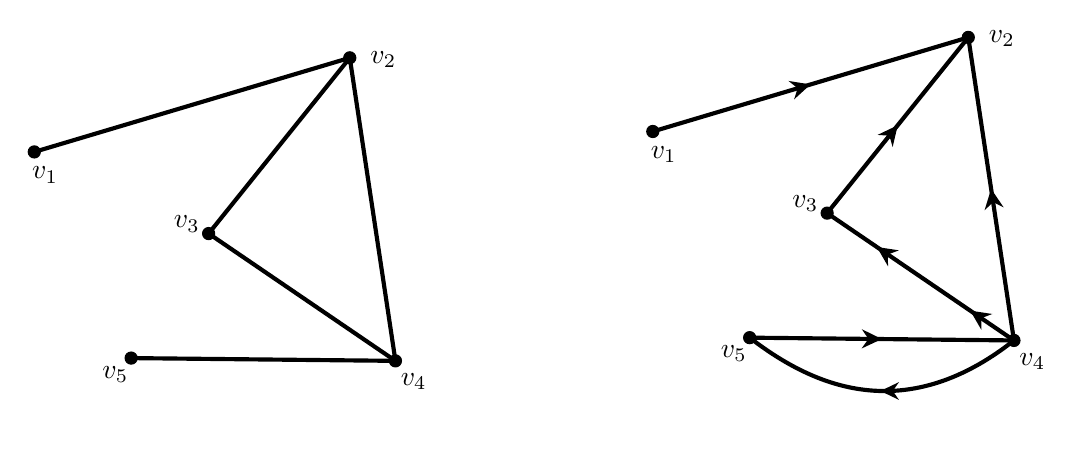
\begin{tikzpicture}[x=0.5pt,y=0.5pt,yscale=-1,xscale=1]
%uncomment if require: \path (0,306); %set diagram left start at 0, and has height of 306

%Flowchart: Connector [id:dp6790201336903005] 
\draw  [fill={rgb, 255:red, 0; green, 0; blue, 0 }  ,fill opacity=1 ] (89,103) .. controls (89,100.58) and (90.96,98.62) .. (93.38,98.62) .. controls (95.79,98.62) and (97.75,100.58) .. (97.75,103) .. controls (97.75,105.42) and (95.79,107.38) .. (93.38,107.38) .. controls (90.96,107.38) and (89,105.42) .. (89,103) -- cycle ;
%Flowchart: Connector [id:dp8323400540036575] 
\draw  [fill={rgb, 255:red, 0; green, 0; blue, 0 }  ,fill opacity=1 ] (317,35) .. controls (317,32.58) and (318.96,30.62) .. (321.38,30.62) .. controls (323.79,30.62) and (325.75,32.58) .. (325.75,35) .. controls (325.75,37.42) and (323.79,39.38) .. (321.38,39.38) .. controls (318.96,39.38) and (317,37.42) .. (317,35) -- cycle ;
%Flowchart: Connector [id:dp4253552390250358] 
\draw  [fill={rgb, 255:red, 0; green, 0; blue, 0 }  ,fill opacity=1 ] (350,254) .. controls (350,251.58) and (351.96,249.62) .. (354.38,249.62) .. controls (356.79,249.62) and (358.75,251.58) .. (358.75,254) .. controls (358.75,256.42) and (356.79,258.38) .. (354.38,258.38) .. controls (351.96,258.38) and (350,256.42) .. (350,254) -- cycle ;
%Flowchart: Connector [id:dp15161486550981407] 
\draw  [fill={rgb, 255:red, 0; green, 0; blue, 0 }  ,fill opacity=1 ] (159,252) .. controls (159,249.58) and (160.96,247.62) .. (163.38,247.62) .. controls (165.79,247.62) and (167.75,249.58) .. (167.75,252) .. controls (167.75,254.42) and (165.79,256.38) .. (163.38,256.38) .. controls (160.96,256.38) and (159,254.42) .. (159,252) -- cycle ;
%Straight Lines [id:da33485918253219815] 
\draw [color={rgb, 255:red, 0; green, 0; blue, 0 }  ,draw opacity=1 ][line width=1.5]    (93.38,103) -- (321.38,35) ;
%Flowchart: Connector [id:dp6607903165665847] 
\draw  [fill={rgb, 255:red, 0; green, 0; blue, 0 }  ,fill opacity=1 ] (215,162) .. controls (215,159.58) and (216.96,157.62) .. (219.38,157.62) .. controls (221.79,157.62) and (223.75,159.58) .. (223.75,162) .. controls (223.75,164.42) and (221.79,166.38) .. (219.38,166.38) .. controls (216.96,166.38) and (215,164.42) .. (215,162) -- cycle ;
%Straight Lines [id:da9704902392723933] 
\draw [color={rgb, 255:red, 0; green, 0; blue, 0 }  ,draw opacity=1 ][line width=1.5]    (219.38,162) -- (321.38,35) ;
%Straight Lines [id:da3214089668075706] 
\draw [color={rgb, 255:red, 0; green, 0; blue, 0 }  ,draw opacity=1 ][line width=1.5]    (163.38,252) -- (354.38,254) ;
%Straight Lines [id:da35660925127636145] 
\draw [color={rgb, 255:red, 0; green, 0; blue, 0 }  ,draw opacity=1 ][line width=1.5]    (354.38,254) -- (321.38,35) ;
%Straight Lines [id:da32904194418935273] 
\draw [color={rgb, 255:red, 0; green, 0; blue, 0 }  ,draw opacity=1 ][line width=1.5]    (354.38,254) -- (219.38,162) ;
%Flowchart: Connector [id:dp12548501893331887] 
\draw  [fill={rgb, 255:red, 0; green, 0; blue, 0 }  ,fill opacity=1 ] (536,88.24) .. controls (536,85.82) and (537.96,83.86) .. (540.38,83.86) .. controls (542.79,83.86) and (544.75,85.82) .. (544.75,88.24) .. controls (544.75,90.65) and (542.79,92.61) .. (540.38,92.61) .. controls (537.96,92.61) and (536,90.65) .. (536,88.24) -- cycle ;
%Flowchart: Connector [id:dp6716572124529165] 
\draw  [fill={rgb, 255:red, 0; green, 0; blue, 0 }  ,fill opacity=1 ] (764,20.24) .. controls (764,17.82) and (765.96,15.86) .. (768.38,15.86) .. controls (770.79,15.86) and (772.75,17.82) .. (772.75,20.24) .. controls (772.75,22.65) and (770.79,24.61) .. (768.38,24.61) .. controls (765.96,24.61) and (764,22.65) .. (764,20.24) -- cycle ;
%Flowchart: Connector [id:dp08043752132546567] 
\draw  [fill={rgb, 255:red, 0; green, 0; blue, 0 }  ,fill opacity=1 ] (797,239.24) .. controls (797,236.82) and (798.96,234.86) .. (801.38,234.86) .. controls (803.79,234.86) and (805.75,236.82) .. (805.75,239.24) .. controls (805.75,241.65) and (803.79,243.61) .. (801.38,243.61) .. controls (798.96,243.61) and (797,241.65) .. (797,239.24) -- cycle ;
%Flowchart: Connector [id:dp2016204031515907] 
\draw  [fill={rgb, 255:red, 0; green, 0; blue, 0 }  ,fill opacity=1 ] (606,237.24) .. controls (606,234.82) and (607.96,232.86) .. (610.38,232.86) .. controls (612.79,232.86) and (614.75,234.82) .. (614.75,237.24) .. controls (614.75,239.65) and (612.79,241.61) .. (610.38,241.61) .. controls (607.96,241.61) and (606,239.65) .. (606,237.24) -- cycle ;
%Straight Lines [id:da9124210665741758] 
\draw [color={rgb, 255:red, 0; green, 0; blue, 0 }  ,draw opacity=1 ][line width=1.5]    (540.38,88.24) -- (768.38,20.24) ;
\draw [shift={(654.38,54.24)}, rotate = 163.39] [fill={rgb, 255:red, 0; green, 0; blue, 0 }  ,fill opacity=1 ][line width=0.08]  [draw opacity=0] (14.56,-6.99) -- (0,0) -- (14.56,6.99) -- (9.67,0) -- cycle    ;
%Flowchart: Connector [id:dp17378293402374523] 
\draw  [fill={rgb, 255:red, 0; green, 0; blue, 0 }  ,fill opacity=1 ] (662,147.24) .. controls (662,144.82) and (663.96,142.86) .. (666.38,142.86) .. controls (668.79,142.86) and (670.75,144.82) .. (670.75,147.24) .. controls (670.75,149.65) and (668.79,151.61) .. (666.38,151.61) .. controls (663.96,151.61) and (662,149.65) .. (662,147.24) -- cycle ;
%Straight Lines [id:da42496408917755524] 
\draw [color={rgb, 255:red, 0; green, 0; blue, 0 }  ,draw opacity=1 ][line width=1.5]    (666.38,147.24) -- (768.38,20.24) ;
\draw [shift={(717.38,83.74)}, rotate = 128.77] [fill={rgb, 255:red, 0; green, 0; blue, 0 }  ,fill opacity=1 ][line width=0.08]  [draw opacity=0] (14.56,-6.99) -- (0,0) -- (14.56,6.99) -- (9.67,0) -- cycle    ;
%Straight Lines [id:da352612778908305] 
\draw [color={rgb, 255:red, 0; green, 0; blue, 0 }  ,draw opacity=1 ][line width=1.5]    (610.38,237.24) -- (801.38,239.24) ;
\draw [shift={(705.88,238.24)}, rotate = 180.6] [fill={rgb, 255:red, 0; green, 0; blue, 0 }  ,fill opacity=1 ][line width=0.08]  [draw opacity=0] (14.56,-6.99) -- (0,0) -- (14.56,6.99) -- (9.67,0) -- cycle    ;
%Straight Lines [id:da014195829977063146] 
\draw [color={rgb, 255:red, 0; green, 0; blue, 0 }  ,draw opacity=1 ][line width=1.5]    (801.38,239.24) -- (768.38,20.24) ;
\draw [shift={(784.88,129.74)}, rotate = 81.43] [fill={rgb, 255:red, 0; green, 0; blue, 0 }  ,fill opacity=1 ][line width=0.08]  [draw opacity=0] (14.56,-6.99) -- (0,0) -- (14.56,6.99) -- (9.67,0) -- cycle    ;
%Straight Lines [id:da2717088403944091] 
\draw [color={rgb, 255:red, 0; green, 0; blue, 0 }  ,draw opacity=1 ][line width=1.5]    (801.38,239.24) -- (738.18,196.17) -- (666.38,147.24) ;
\draw [shift={(769.78,217.7)}, rotate = 34.27] [fill={rgb, 255:red, 0; green, 0; blue, 0 }  ,fill opacity=1 ][line width=0.08]  [draw opacity=0] (14.56,-6.99) -- (0,0) -- (14.56,6.99) -- (9.67,0) -- cycle    ;
\draw [shift={(702.28,171.7)}, rotate = 34.27] [fill={rgb, 255:red, 0; green, 0; blue, 0 }  ,fill opacity=1 ][line width=0.08]  [draw opacity=0] (14.56,-6.99) -- (0,0) -- (14.56,6.99) -- (9.67,0) -- cycle    ;
%Curve Lines [id:da5145213870577791] 
\draw [line width=1.5]    (801.38,239.24) .. controls (719.63,303.76) and (652.63,269.76) .. (610.38,237.24) ;
\draw [shift={(704.9,275.77)}, rotate = 0.02] [fill={rgb, 255:red, 0; green, 0; blue, 0 }  ][line width=0.08]  [draw opacity=0] (13.4,-6.43) -- (0,0) -- (13.4,6.44) -- (8.9,0) -- cycle    ;

% Text Node
\draw (90,112) node [anchor=north west][inner sep=0.75pt]   [align=left] {$\displaystyle v_{1}$};
% Text Node
\draw (192.38,147.38) node [anchor=north west][inner sep=0.75pt]   [align=left] {$\displaystyle v_{3}$};
% Text Node
\draw (140.75,256) node [anchor=north west][inner sep=0.75pt]   [align=left] {$\displaystyle v_{5}$};
% Text Node
\draw (356.38,261.38) node [anchor=north west][inner sep=0.75pt]   [align=left] {$\displaystyle v_{4}$};
% Text Node
\draw (334.38,28.38) node [anchor=north west][inner sep=0.75pt]   [align=left] {$\displaystyle v_{2}$};
% Text Node
\draw (537,97.24) node [anchor=north west][inner sep=0.75pt]   [align=left] {$\displaystyle v_{1}$};
% Text Node
\draw (639.38,132.61) node [anchor=north west][inner sep=0.75pt]   [align=left] {$\displaystyle v_{3}$};
% Text Node
\draw (587.75,241.24) node [anchor=north west][inner sep=0.75pt]   [align=left] {$\displaystyle v_{5}$};
% Text Node
\draw (803.38,246.61) node [anchor=north west][inner sep=0.75pt]   [align=left] {$\displaystyle v_{4}$};
% Text Node
\draw (781.38,13.61) node [anchor=north west][inner sep=0.75pt]   [align=left] {$\displaystyle v_{2}$};


\end{tikzpicture}
}
\caption{Left: a undirected graph $G = (V, E)$, where $V = \{v_1, v_2, v_3, v_4, v_5\}$,
and $E = \{(v_1, v_2), (v_3, v_2), (v_4, v_3), (v_4, v_2), (v_4, v_5)\}$.
Right: a directed graph $G = (V, E)$, where $V = \{v_1, v_2, v_3, v_4, v_5\}$,
and $E = \{(v_1, v_2), (v_3, v_2), (v_4, v_3), (v_4, v_2), (v_4, v_5), (v_5, v_4)\}$.}
\label{fig:graphs}
\end{figure}

Notice that for an edge $(v_i, v_j)$ in an undirected graph, the order of $v_i$ and $v_j$ are interchangable,
i.e., $(v_i, v_j) = (v_j, v_i)$. In directed graph this is not the case.

%An undirected graph $G = (V, E)$ can be transformed into a directed graph $G' = (V, E')$ by replacing an (undirected) edge $(v_i, v_j) \in E$ as two (directed) edges $(v_i, v_j)$ and $(v_j, v_i)$ in $E'$.

Adjacency matrix and adjacency list are two commonly-used data structures to represent a graph.
Adjacency matrix uses a binary matrix $M$ of size $|V|\times |V|$ to store a graph $G = (V, E)$:
$M[i,j] = 1$ if and only if $(v_i, v_j) \in E$. This definition applies to both directed graphs and undirected graphs.

For undirected graphs, clearly the adjacency matrix $M$ is symmetric. 
If we assume that there is no ``self-loop'' edges in the form of $(v_i, v_i)$, 
then the number of ``1''s in $M$ is exactly $2|E|$ for undirected graph.
The number of ``1''s in $M$ is exactly $|E|$ for directed graph. 

\begin{figure}[h!]
\centering{

\tikzset{every picture/.style={line width=0.75pt}} %set default line width to 0.75pt        

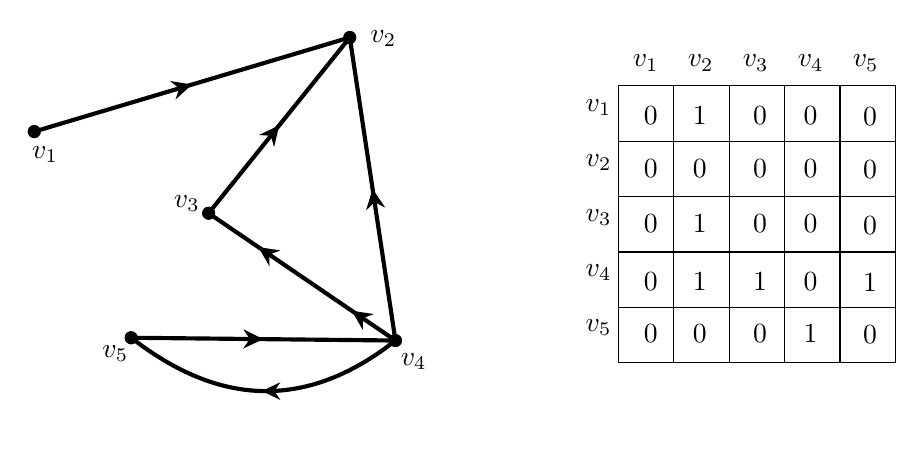
\begin{tikzpicture}[x=0.5pt,y=0.5pt,yscale=-1,xscale=1]
%uncomment if require: \path (0,299); %set diagram left start at 0, and has height of 299

%Flowchart: Connector [id:dp14554034773886415] 
\draw  [fill={rgb, 255:red, 0; green, 0; blue, 0 }  ,fill opacity=1 ] (25,96) .. controls (25,93.58) and (26.96,91.62) .. (29.38,91.62) .. controls (31.79,91.62) and (33.75,93.58) .. (33.75,96) .. controls (33.75,98.42) and (31.79,100.38) .. (29.38,100.38) .. controls (26.96,100.38) and (25,98.42) .. (25,96) -- cycle ;
%Flowchart: Connector [id:dp7796394659617965] 
\draw  [fill={rgb, 255:red, 0; green, 0; blue, 0 }  ,fill opacity=1 ] (253,28) .. controls (253,25.58) and (254.96,23.62) .. (257.38,23.62) .. controls (259.79,23.62) and (261.75,25.58) .. (261.75,28) .. controls (261.75,30.42) and (259.79,32.38) .. (257.38,32.38) .. controls (254.96,32.38) and (253,30.42) .. (253,28) -- cycle ;
%Flowchart: Connector [id:dp8410872532958124] 
\draw  [fill={rgb, 255:red, 0; green, 0; blue, 0 }  ,fill opacity=1 ] (286,247) .. controls (286,244.58) and (287.96,242.62) .. (290.38,242.62) .. controls (292.79,242.62) and (294.75,244.58) .. (294.75,247) .. controls (294.75,249.42) and (292.79,251.38) .. (290.38,251.38) .. controls (287.96,251.38) and (286,249.42) .. (286,247) -- cycle ;
%Flowchart: Connector [id:dp17196535593949425] 
\draw  [fill={rgb, 255:red, 0; green, 0; blue, 0 }  ,fill opacity=1 ] (95,245) .. controls (95,242.58) and (96.96,240.62) .. (99.38,240.62) .. controls (101.79,240.62) and (103.75,242.58) .. (103.75,245) .. controls (103.75,247.42) and (101.79,249.38) .. (99.38,249.38) .. controls (96.96,249.38) and (95,247.42) .. (95,245) -- cycle ;
%Straight Lines [id:da7073971572516686] 
\draw [color={rgb, 255:red, 0; green, 0; blue, 0 }  ,draw opacity=1 ][line width=1.5]    (29.38,96) -- (257.38,28) ;
\draw [shift={(143.38,62)}, rotate = 523.39] [fill={rgb, 255:red, 0; green, 0; blue, 0 }  ,fill opacity=1 ][line width=0.08]  [draw opacity=0] (14.56,-6.99) -- (0,0) -- (14.56,6.99) -- (9.67,0) -- cycle    ;
%Flowchart: Connector [id:dp6372189195472704] 
\draw  [fill={rgb, 255:red, 0; green, 0; blue, 0 }  ,fill opacity=1 ] (151,155) .. controls (151,152.58) and (152.96,150.62) .. (155.38,150.62) .. controls (157.79,150.62) and (159.75,152.58) .. (159.75,155) .. controls (159.75,157.42) and (157.79,159.38) .. (155.38,159.38) .. controls (152.96,159.38) and (151,157.42) .. (151,155) -- cycle ;
%Straight Lines [id:da6054846048754496] 
\draw [color={rgb, 255:red, 0; green, 0; blue, 0 }  ,draw opacity=1 ][line width=1.5]    (155.38,155) -- (257.38,28) ;
\draw [shift={(206.38,91.5)}, rotate = 488.77] [fill={rgb, 255:red, 0; green, 0; blue, 0 }  ,fill opacity=1 ][line width=0.08]  [draw opacity=0] (14.56,-6.99) -- (0,0) -- (14.56,6.99) -- (9.67,0) -- cycle    ;
%Straight Lines [id:da8238439208450634] 
\draw [color={rgb, 255:red, 0; green, 0; blue, 0 }  ,draw opacity=1 ][line width=1.5]    (99.38,245) -- (290.38,247) ;
\draw [shift={(194.88,246)}, rotate = 180.6] [fill={rgb, 255:red, 0; green, 0; blue, 0 }  ,fill opacity=1 ][line width=0.08]  [draw opacity=0] (14.56,-6.99) -- (0,0) -- (14.56,6.99) -- (9.67,0) -- cycle    ;
%Straight Lines [id:da4336320329770583] 
\draw [color={rgb, 255:red, 0; green, 0; blue, 0 }  ,draw opacity=1 ][line width=1.5]    (290.38,247) -- (257.38,28) ;
\draw [shift={(273.88,137.5)}, rotate = 441.43] [fill={rgb, 255:red, 0; green, 0; blue, 0 }  ,fill opacity=1 ][line width=0.08]  [draw opacity=0] (14.56,-6.99) -- (0,0) -- (14.56,6.99) -- (9.67,0) -- cycle    ;
%Straight Lines [id:da684522286123465] 
\draw [color={rgb, 255:red, 0; green, 0; blue, 0 }  ,draw opacity=1 ][line width=1.5]    (290.38,247) -- (227.18,203.93) -- (155.38,155) ;
\draw [shift={(258.78,225.47)}, rotate = 394.27] [fill={rgb, 255:red, 0; green, 0; blue, 0 }  ,fill opacity=1 ][line width=0.08]  [draw opacity=0] (14.56,-6.99) -- (0,0) -- (14.56,6.99) -- (9.67,0) -- cycle    ;
\draw [shift={(191.28,179.47)}, rotate = 394.27] [fill={rgb, 255:red, 0; green, 0; blue, 0 }  ,fill opacity=1 ][line width=0.08]  [draw opacity=0] (14.56,-6.99) -- (0,0) -- (14.56,6.99) -- (9.67,0) -- cycle    ;
%Curve Lines [id:da7415875935631565] 
\draw [line width=1.5]    (290.38,247) .. controls (208.63,311.52) and (141.63,277.52) .. (99.38,245) ;
\draw [shift={(193.9,283.53)}, rotate = 360.02] [fill={rgb, 255:red, 0; green, 0; blue, 0 }  ][line width=0.08]  [draw opacity=0] (13.4,-6.43) -- (0,0) -- (13.4,6.44) -- (8.9,0) -- cycle    ;
%Shape: Grid [id:dp07332615829400024] 
\draw  [draw opacity=0] (651.64,63) -- (451.64,63) -- (451.64,263) -- (651.64,263) -- cycle ; \draw   (611.64,63) -- (611.64,263)(571.64,63) -- (571.64,263)(531.64,63) -- (531.64,263)(491.64,63) -- (491.64,263) ; \draw   (651.64,103) -- (451.64,103)(651.64,143) -- (451.64,143)(651.64,183) -- (451.64,183)(651.64,223) -- (451.64,223) ; \draw   (651.64,63) -- (451.64,63) -- (451.64,263) -- (651.64,263) -- cycle ;

% Text Node
\draw (26,104.93) node [anchor=north west][inner sep=0.75pt]   [align=left] {$\displaystyle v_{1}$};
% Text Node
\draw (128.38,140.31) node [anchor=north west][inner sep=0.75pt]   [align=left] {$\displaystyle v_{3}$};
% Text Node
\draw (76.75,248.93) node [anchor=north west][inner sep=0.75pt]   [align=left] {$\displaystyle v_{5}$};
% Text Node
\draw (292.38,254.31) node [anchor=north west][inner sep=0.75pt]   [align=left] {$\displaystyle v_{4}$};
% Text Node
\draw (270.38,21.31) node [anchor=north west][inner sep=0.75pt]   [align=left] {$\displaystyle v_{2}$};
% Text Node
\draw (426,70.93) node [anchor=north west][inner sep=0.75pt]   [align=left] {$\displaystyle v_{1}$};
% Text Node
\draw (426,110.68) node [anchor=north west][inner sep=0.75pt]   [align=left] {$\displaystyle v_{2}$};
% Text Node
\draw (426,150.43) node [anchor=north west][inner sep=0.75pt]   [align=left] {$\displaystyle v_{3}$};
% Text Node
\draw (426,190.18) node [anchor=north west][inner sep=0.75pt]   [align=left] {$\displaystyle v_{4}$};
% Text Node
\draw (426,229.93) node [anchor=north west][inner sep=0.75pt]   [align=left] {$\displaystyle v_{5}$};
% Text Node
\draw (460,38.81) node [anchor=north west][inner sep=0.75pt]   [align=left] {$\displaystyle v_{1}$};
% Text Node
\draw (499.75,38.81) node [anchor=north west][inner sep=0.75pt]   [align=left] {$\displaystyle v_{2}$};
% Text Node
\draw (539.5,38.81) node [anchor=north west][inner sep=0.75pt]   [align=left] {$\displaystyle v_{3}$};
% Text Node
\draw (579.25,38.81) node [anchor=north west][inner sep=0.75pt]   [align=left] {$\displaystyle v_{4}$};
% Text Node
\draw (619,38.81) node [anchor=north west][inner sep=0.75pt]   [align=left] {$\displaystyle v_{5}$};
% Text Node
\draw (503.5,75.93) node [anchor=north west][inner sep=0.75pt]   [align=left] {$\displaystyle 1$};
% Text Node
\draw (503.5,195.93) node [anchor=north west][inner sep=0.75pt]   [align=left] {$\displaystyle 1$};
% Text Node
\draw (503.5,154.43) node [anchor=north west][inner sep=0.75pt]   [align=left] {$\displaystyle 1$};
% Text Node
\draw (547,195.93) node [anchor=north west][inner sep=0.75pt]   [align=left] {$\displaystyle 1$};
% Text Node
\draw (626.5,196.93) node [anchor=north west][inner sep=0.75pt]   [align=left] {$\displaystyle 1$};
% Text Node
\draw (583.5,233.43) node [anchor=north west][inner sep=0.75pt]   [align=left] {$\displaystyle 1$};
% Text Node
\draw (468,75.93) node [anchor=north west][inner sep=0.75pt]   [align=left] {$\displaystyle 0$};
% Text Node
\draw (626.5,115.43) node [anchor=north west][inner sep=0.75pt]   [align=left] {$\displaystyle 0$};
% Text Node
\draw (583.5,114.43) node [anchor=north west][inner sep=0.75pt]   [align=left] {$\displaystyle 0$};
% Text Node
\draw (547,75.93) node [anchor=north west][inner sep=0.75pt]   [align=left] {$\displaystyle 0$};
% Text Node
\draw (583.5,75.93) node [anchor=north west][inner sep=0.75pt]   [align=left] {$\displaystyle 0$};
% Text Node
\draw (626.5,76.93) node [anchor=north west][inner sep=0.75pt]   [align=left] {$\displaystyle 0$};
% Text Node
\draw (468,114.43) node [anchor=north west][inner sep=0.75pt]   [align=left] {$\displaystyle 0$};
% Text Node
\draw (503.5,114.43) node [anchor=north west][inner sep=0.75pt]   [align=left] {$\displaystyle 0$};
% Text Node
\draw (547,114.43) node [anchor=north west][inner sep=0.75pt]   [align=left] {$\displaystyle 0$};
% Text Node
\draw (626.5,155.43) node [anchor=north west][inner sep=0.75pt]   [align=left] {$\displaystyle 0$};
% Text Node
\draw (583.5,154.43) node [anchor=north west][inner sep=0.75pt]   [align=left] {$\displaystyle 0$};
% Text Node
\draw (547,154.43) node [anchor=north west][inner sep=0.75pt]   [align=left] {$\displaystyle 0$};
% Text Node
\draw (547,233.43) node [anchor=north west][inner sep=0.75pt]   [align=left] {$\displaystyle 0$};
% Text Node
\draw (503.5,233.43) node [anchor=north west][inner sep=0.75pt]   [align=left] {$\displaystyle 0$};
% Text Node
\draw (468,233.43) node [anchor=north west][inner sep=0.75pt]   [align=left] {$\displaystyle 0$};
% Text Node
\draw (468,154.43) node [anchor=north west][inner sep=0.75pt]   [align=left] {$\displaystyle 0$};
% Text Node
\draw (468,195.93) node [anchor=north west][inner sep=0.75pt]   [align=left] {$\displaystyle 0$};
% Text Node
\draw (583.5,195.93) node [anchor=north west][inner sep=0.75pt]   [align=left] {$\displaystyle 0$};
% Text Node
\draw (626.5,234.43) node [anchor=north west][inner sep=0.75pt]   [align=left] {$\displaystyle 0$};


\end{tikzpicture}

}
\caption{Adjacency matrix representation~(directed graph).}
\end{figure}

\begin{figure}[h!]
\centering{

\tikzset{every picture/.style={line width=0.75pt}} %set default line width to 0.75pt        

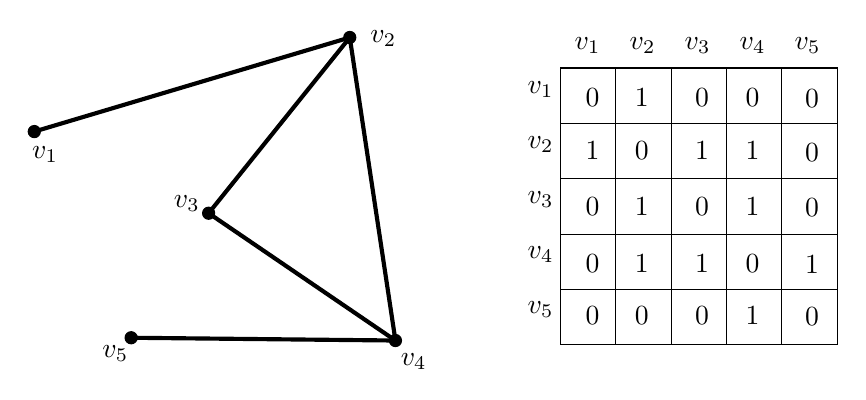
\begin{tikzpicture}[x=0.5pt,y=0.5pt,yscale=-1,xscale=1]
%uncomment if require: \path (0,306); %set diagram left start at 0, and has height of 306

%Flowchart: Connector [id:dp14554034773886415] 
\draw  [fill={rgb, 255:red, 0; green, 0; blue, 0 }  ,fill opacity=1 ] (25,96) .. controls (25,93.58) and (26.96,91.62) .. (29.38,91.62) .. controls (31.79,91.62) and (33.75,93.58) .. (33.75,96) .. controls (33.75,98.42) and (31.79,100.38) .. (29.38,100.38) .. controls (26.96,100.38) and (25,98.42) .. (25,96) -- cycle ;
%Flowchart: Connector [id:dp7796394659617965] 
\draw  [fill={rgb, 255:red, 0; green, 0; blue, 0 }  ,fill opacity=1 ] (253,28) .. controls (253,25.58) and (254.96,23.62) .. (257.38,23.62) .. controls (259.79,23.62) and (261.75,25.58) .. (261.75,28) .. controls (261.75,30.42) and (259.79,32.38) .. (257.38,32.38) .. controls (254.96,32.38) and (253,30.42) .. (253,28) -- cycle ;
%Flowchart: Connector [id:dp8410872532958124] 
\draw  [fill={rgb, 255:red, 0; green, 0; blue, 0 }  ,fill opacity=1 ] (286,247) .. controls (286,244.58) and (287.96,242.62) .. (290.38,242.62) .. controls (292.79,242.62) and (294.75,244.58) .. (294.75,247) .. controls (294.75,249.42) and (292.79,251.38) .. (290.38,251.38) .. controls (287.96,251.38) and (286,249.42) .. (286,247) -- cycle ;
%Flowchart: Connector [id:dp17196535593949425] 
\draw  [fill={rgb, 255:red, 0; green, 0; blue, 0 }  ,fill opacity=1 ] (95,245) .. controls (95,242.58) and (96.96,240.62) .. (99.38,240.62) .. controls (101.79,240.62) and (103.75,242.58) .. (103.75,245) .. controls (103.75,247.42) and (101.79,249.38) .. (99.38,249.38) .. controls (96.96,249.38) and (95,247.42) .. (95,245) -- cycle ;
%Straight Lines [id:da7073971572516686] 
\draw [color={rgb, 255:red, 0; green, 0; blue, 0 }  ,draw opacity=1 ][line width=1.5]    (29.38,96) -- (257.38,28) ;
%Flowchart: Connector [id:dp6372189195472704] 
\draw  [fill={rgb, 255:red, 0; green, 0; blue, 0 }  ,fill opacity=1 ] (151,155) .. controls (151,152.58) and (152.96,150.62) .. (155.38,150.62) .. controls (157.79,150.62) and (159.75,152.58) .. (159.75,155) .. controls (159.75,157.42) and (157.79,159.38) .. (155.38,159.38) .. controls (152.96,159.38) and (151,157.42) .. (151,155) -- cycle ;
%Straight Lines [id:da6054846048754496] 
\draw [color={rgb, 255:red, 0; green, 0; blue, 0 }  ,draw opacity=1 ][line width=1.5]    (155.38,155) -- (257.38,28) ;
%Straight Lines [id:da8238439208450634] 
\draw [color={rgb, 255:red, 0; green, 0; blue, 0 }  ,draw opacity=1 ][line width=1.5]    (99.38,245) -- (290.38,247) ;
%Straight Lines [id:da4336320329770583] 
\draw [color={rgb, 255:red, 0; green, 0; blue, 0 }  ,draw opacity=1 ][line width=1.5]    (290.38,247) -- (257.38,28) ;
%Straight Lines [id:da684522286123465] 
\draw [color={rgb, 255:red, 0; green, 0; blue, 0 }  ,draw opacity=1 ][line width=1.5]    (290.38,247) -- (155.38,155) ;
%Shape: Grid [id:dp16853858164363344] 
\draw  [draw opacity=0] (609.64,50.09) -- (409.64,50.09) -- (409.64,250.09) -- (609.64,250.09) -- cycle ; \draw   (569.64,50.09) -- (569.64,250.09)(529.64,50.09) -- (529.64,250.09)(489.64,50.09) -- (489.64,250.09)(449.64,50.09) -- (449.64,250.09) ; \draw   (609.64,90.09) -- (409.64,90.09)(609.64,130.09) -- (409.64,130.09)(609.64,170.09) -- (409.64,170.09)(609.64,210.09) -- (409.64,210.09) ; \draw   (609.64,50.09) -- (409.64,50.09) -- (409.64,250.09) -- (609.64,250.09) -- cycle ;

% Text Node
\draw (26,104.93) node [anchor=north west][inner sep=0.75pt]   [align=left] {$\displaystyle v_{1}$};
% Text Node
\draw (128.38,140.31) node [anchor=north west][inner sep=0.75pt]   [align=left] {$\displaystyle v_{3}$};
% Text Node
\draw (76.75,248.93) node [anchor=north west][inner sep=0.75pt]   [align=left] {$\displaystyle v_{5}$};
% Text Node
\draw (292.38,254.31) node [anchor=north west][inner sep=0.75pt]   [align=left] {$\displaystyle v_{4}$};
% Text Node
\draw (270.38,21.31) node [anchor=north west][inner sep=0.75pt]   [align=left] {$\displaystyle v_{2}$};
% Text Node
\draw (384,58.03) node [anchor=north west][inner sep=0.75pt]   [align=left] {$\displaystyle v_{1}$};
% Text Node
\draw (384,97.78) node [anchor=north west][inner sep=0.75pt]   [align=left] {$\displaystyle v_{2}$};
% Text Node
\draw (384,137.53) node [anchor=north west][inner sep=0.75pt]   [align=left] {$\displaystyle v_{3}$};
% Text Node
\draw (384,177.28) node [anchor=north west][inner sep=0.75pt]   [align=left] {$\displaystyle v_{4}$};
% Text Node
\draw (384,217.03) node [anchor=north west][inner sep=0.75pt]   [align=left] {$\displaystyle v_{5}$};
% Text Node
\draw (418,25.9) node [anchor=north west][inner sep=0.75pt]   [align=left] {$\displaystyle v_{1}$};
% Text Node
\draw (457.75,25.9) node [anchor=north west][inner sep=0.75pt]   [align=left] {$\displaystyle v_{2}$};
% Text Node
\draw (497.5,25.9) node [anchor=north west][inner sep=0.75pt]   [align=left] {$\displaystyle v_{3}$};
% Text Node
\draw (537.25,25.9) node [anchor=north west][inner sep=0.75pt]   [align=left] {$\displaystyle v_{4}$};
% Text Node
\draw (577,25.9) node [anchor=north west][inner sep=0.75pt]   [align=left] {$\displaystyle v_{5}$};
% Text Node
\draw (461.5,63.03) node [anchor=north west][inner sep=0.75pt]   [align=left] {$\displaystyle 1$};
% Text Node
\draw (461.5,183.03) node [anchor=north west][inner sep=0.75pt]   [align=left] {$\displaystyle 1$};
% Text Node
\draw (461.5,141.53) node [anchor=north west][inner sep=0.75pt]   [align=left] {$\displaystyle 1$};
% Text Node
\draw (505,183.03) node [anchor=north west][inner sep=0.75pt]   [align=left] {$\displaystyle 1$};
% Text Node
\draw (584.5,184.03) node [anchor=north west][inner sep=0.75pt]   [align=left] {$\displaystyle 1$};
% Text Node
\draw (541.5,220.53) node [anchor=north west][inner sep=0.75pt]   [align=left] {$\displaystyle 1$};
% Text Node
\draw (426,63.03) node [anchor=north west][inner sep=0.75pt]   [align=left] {$\displaystyle 0$};
% Text Node
\draw (584.5,102.53) node [anchor=north west][inner sep=0.75pt]   [align=left] {$\displaystyle 0$};
% Text Node
\draw (541.5,101.53) node [anchor=north west][inner sep=0.75pt]   [align=left] {$\displaystyle 1$};
% Text Node
\draw (505,63.03) node [anchor=north west][inner sep=0.75pt]   [align=left] {$\displaystyle 0$};
% Text Node
\draw (541.5,63.03) node [anchor=north west][inner sep=0.75pt]   [align=left] {$\displaystyle 0$};
% Text Node
\draw (584.5,64.03) node [anchor=north west][inner sep=0.75pt]   [align=left] {$\displaystyle 0$};
% Text Node
\draw (426,101.53) node [anchor=north west][inner sep=0.75pt]   [align=left] {$\displaystyle 1$};
% Text Node
\draw (461.5,101.53) node [anchor=north west][inner sep=0.75pt]   [align=left] {$\displaystyle 0$};
% Text Node
\draw (505,101.53) node [anchor=north west][inner sep=0.75pt]   [align=left] {$\displaystyle 1$};
% Text Node
\draw (584.5,142.53) node [anchor=north west][inner sep=0.75pt]   [align=left] {$\displaystyle 0$};
% Text Node
\draw (541.5,141.53) node [anchor=north west][inner sep=0.75pt]   [align=left] {$\displaystyle 1$};
% Text Node
\draw (505,141.53) node [anchor=north west][inner sep=0.75pt]   [align=left] {$\displaystyle 0$};
% Text Node
\draw (505,220.53) node [anchor=north west][inner sep=0.75pt]   [align=left] {$\displaystyle 0$};
% Text Node
\draw (461.5,220.53) node [anchor=north west][inner sep=0.75pt]   [align=left] {$\displaystyle 0$};
% Text Node
\draw (426,220.53) node [anchor=north west][inner sep=0.75pt]   [align=left] {$\displaystyle 0$};
% Text Node
\draw (426,141.53) node [anchor=north west][inner sep=0.75pt]   [align=left] {$\displaystyle 0$};
% Text Node
\draw (426,183.03) node [anchor=north west][inner sep=0.75pt]   [align=left] {$\displaystyle 0$};
% Text Node
\draw (541.5,183.03) node [anchor=north west][inner sep=0.75pt]   [align=left] {$\displaystyle 0$};
% Text Node
\draw (584.5,221.53) node [anchor=north west][inner sep=0.75pt]   [align=left] {$\displaystyle 0$};


\end{tikzpicture}

}
\caption{Adjacency matrix representation~(undirected graph).}
\end{figure}

Adjacency list maintains a list/array $A_i$ for each vertex $v_i \in V$, where
$A_i$ stores $\{v_j \in V \mid (v_i, v_j) \in E\}$, i.e., the adjacent edges/vertices of $v_i$.
A pointer is usually maintained for each vertex $v_i$ that points to the array $A_i$.
Clearly, for undirected graph, $\sum_{v_i \in V} |A_i| = 2|E|$, assuming that there is no ``self-loop'' edges.
For directed graph, $\sum_{v_i \in V} |A_i| = |E|$.

\begin{figure}[h!]
\centering{

\tikzset{every picture/.style={line width=0.75pt}} %set default line width to 0.75pt        

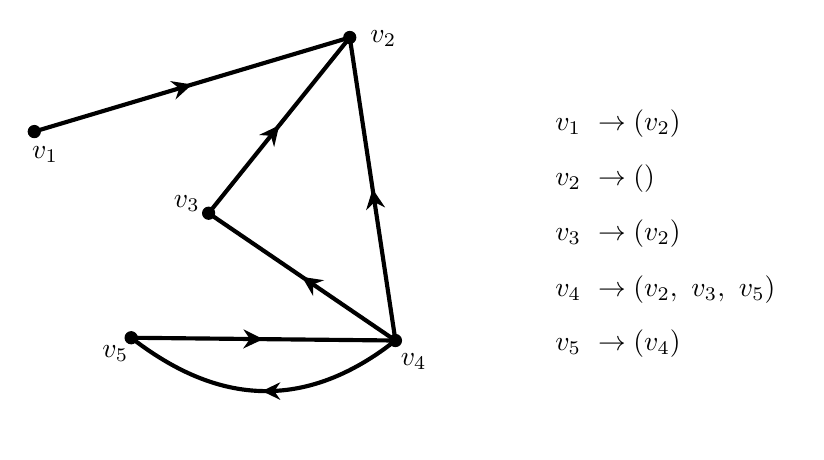
\begin{tikzpicture}[x=0.5pt,y=0.5pt,yscale=-1,xscale=1]
%uncomment if require: \path (0,299); %set diagram left start at 0, and has height of 299

%Flowchart: Connector [id:dp14554034773886415] 
\draw  [fill={rgb, 255:red, 0; green, 0; blue, 0 }  ,fill opacity=1 ] (25,96) .. controls (25,93.58) and (26.96,91.62) .. (29.38,91.62) .. controls (31.79,91.62) and (33.75,93.58) .. (33.75,96) .. controls (33.75,98.42) and (31.79,100.38) .. (29.38,100.38) .. controls (26.96,100.38) and (25,98.42) .. (25,96) -- cycle ;
%Flowchart: Connector [id:dp7796394659617965] 
\draw  [fill={rgb, 255:red, 0; green, 0; blue, 0 }  ,fill opacity=1 ] (253,28) .. controls (253,25.58) and (254.96,23.62) .. (257.38,23.62) .. controls (259.79,23.62) and (261.75,25.58) .. (261.75,28) .. controls (261.75,30.42) and (259.79,32.38) .. (257.38,32.38) .. controls (254.96,32.38) and (253,30.42) .. (253,28) -- cycle ;
%Flowchart: Connector [id:dp8410872532958124] 
\draw  [fill={rgb, 255:red, 0; green, 0; blue, 0 }  ,fill opacity=1 ] (286,247) .. controls (286,244.58) and (287.96,242.62) .. (290.38,242.62) .. controls (292.79,242.62) and (294.75,244.58) .. (294.75,247) .. controls (294.75,249.42) and (292.79,251.38) .. (290.38,251.38) .. controls (287.96,251.38) and (286,249.42) .. (286,247) -- cycle ;
%Flowchart: Connector [id:dp17196535593949425] 
\draw  [fill={rgb, 255:red, 0; green, 0; blue, 0 }  ,fill opacity=1 ] (95,245) .. controls (95,242.58) and (96.96,240.62) .. (99.38,240.62) .. controls (101.79,240.62) and (103.75,242.58) .. (103.75,245) .. controls (103.75,247.42) and (101.79,249.38) .. (99.38,249.38) .. controls (96.96,249.38) and (95,247.42) .. (95,245) -- cycle ;
%Straight Lines [id:da7073971572516686] 
\draw [color={rgb, 255:red, 0; green, 0; blue, 0 }  ,draw opacity=1 ][line width=1.5]    (29.38,96) -- (257.38,28) ;
\draw [shift={(143.38,62)}, rotate = 523.39] [fill={rgb, 255:red, 0; green, 0; blue, 0 }  ,fill opacity=1 ][line width=0.08]  [draw opacity=0] (14.56,-6.99) -- (0,0) -- (14.56,6.99) -- (9.67,0) -- cycle    ;
%Flowchart: Connector [id:dp6372189195472704] 
\draw  [fill={rgb, 255:red, 0; green, 0; blue, 0 }  ,fill opacity=1 ] (151,155) .. controls (151,152.58) and (152.96,150.62) .. (155.38,150.62) .. controls (157.79,150.62) and (159.75,152.58) .. (159.75,155) .. controls (159.75,157.42) and (157.79,159.38) .. (155.38,159.38) .. controls (152.96,159.38) and (151,157.42) .. (151,155) -- cycle ;
%Straight Lines [id:da6054846048754496] 
\draw [color={rgb, 255:red, 0; green, 0; blue, 0 }  ,draw opacity=1 ][line width=1.5]    (155.38,155) -- (257.38,28) ;
\draw [shift={(206.38,91.5)}, rotate = 488.77] [fill={rgb, 255:red, 0; green, 0; blue, 0 }  ,fill opacity=1 ][line width=0.08]  [draw opacity=0] (14.56,-6.99) -- (0,0) -- (14.56,6.99) -- (9.67,0) -- cycle    ;
%Straight Lines [id:da8238439208450634] 
\draw [color={rgb, 255:red, 0; green, 0; blue, 0 }  ,draw opacity=1 ][line width=1.5]    (99.38,245) -- (290.38,247) ;
\draw [shift={(194.88,246)}, rotate = 180.6] [fill={rgb, 255:red, 0; green, 0; blue, 0 }  ,fill opacity=1 ][line width=0.08]  [draw opacity=0] (14.56,-6.99) -- (0,0) -- (14.56,6.99) -- (9.67,0) -- cycle    ;
%Straight Lines [id:da4336320329770583] 
\draw [color={rgb, 255:red, 0; green, 0; blue, 0 }  ,draw opacity=1 ][line width=1.5]    (290.38,247) -- (257.38,28) ;
\draw [shift={(273.88,137.5)}, rotate = 441.43] [fill={rgb, 255:red, 0; green, 0; blue, 0 }  ,fill opacity=1 ][line width=0.08]  [draw opacity=0] (14.56,-6.99) -- (0,0) -- (14.56,6.99) -- (9.67,0) -- cycle    ;
%Curve Lines [id:da7415875935631565] 
\draw [line width=1.5]    (290.38,247) .. controls (208.63,311.52) and (141.63,277.52) .. (99.38,245) ;
\draw [shift={(193.9,283.53)}, rotate = 360.02] [fill={rgb, 255:red, 0; green, 0; blue, 0 }  ][line width=0.08]  [draw opacity=0] (13.4,-6.43) -- (0,0) -- (13.4,6.44) -- (8.9,0) -- cycle    ;
%Straight Lines [id:da6848704742122639] 
\draw [color={rgb, 255:red, 0; green, 0; blue, 0 }  ,draw opacity=1 ][line width=1.5]    (290.38,247) -- (155.38,155) ;
\draw [shift={(222.88,201)}, rotate = 394.27] [fill={rgb, 255:red, 0; green, 0; blue, 0 }  ,fill opacity=1 ][line width=0.08]  [draw opacity=0] (14.56,-6.99) -- (0,0) -- (14.56,6.99) -- (9.67,0) -- cycle    ;

% Text Node
\draw (26,104.93) node [anchor=north west][inner sep=0.75pt]   [align=left] {$\displaystyle v_{1}$};
% Text Node
\draw (128.38,140.31) node [anchor=north west][inner sep=0.75pt]   [align=left] {$\displaystyle v_{3}$};
% Text Node
\draw (76.75,248.93) node [anchor=north west][inner sep=0.75pt]   [align=left] {$\displaystyle v_{5}$};
% Text Node
\draw (292.38,254.31) node [anchor=north west][inner sep=0.75pt]   [align=left] {$\displaystyle v_{4}$};
% Text Node
\draw (270.38,21.31) node [anchor=north west][inner sep=0.75pt]   [align=left] {$\displaystyle v_{2}$};
% Text Node
\draw (404,78.03) node [anchor=north west][inner sep=0.75pt]   [align=left] {$\displaystyle v_{1} \ \rightarrow ( v_{2})$};
% Text Node
\draw (404,117.78) node [anchor=north west][inner sep=0.75pt]   [align=left] {$\displaystyle v_{2} \ \rightarrow ()$};
% Text Node
\draw (404,157.53) node [anchor=north west][inner sep=0.75pt]   [align=left] {$\displaystyle v_{3} \ \rightarrow ( v_{2})$};
% Text Node
\draw (404,198.28) node [anchor=north west][inner sep=0.75pt]   [align=left] {$\displaystyle v_{4} \ \rightarrow ( v_{2} ,\ v_{3} ,\ v_{5})$ \ };
% Text Node
\draw (404,237.03) node [anchor=north west][inner sep=0.75pt]   [align=left] {$\displaystyle v_{5} \ \rightarrow ( v_{4})$};


\end{tikzpicture}

}
\caption{Adjacency list representation~(directed graph).}
\end{figure}

\begin{figure}[h!]
\centering{

\tikzset{every picture/.style={line width=0.75pt}} %set default line width to 0.75pt        

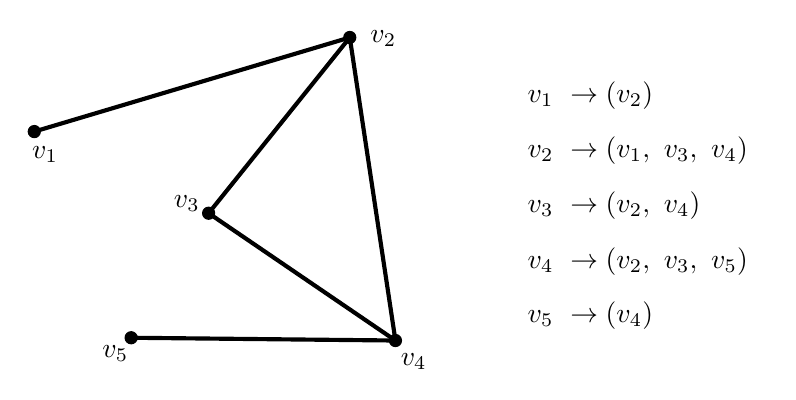
\begin{tikzpicture}[x=0.5pt,y=0.5pt,yscale=-1,xscale=1]
%uncomment if require: \path (0,285); %set diagram left start at 0, and has height of 285

%Flowchart: Connector [id:dp14554034773886415] 
\draw  [fill={rgb, 255:red, 0; green, 0; blue, 0 }  ,fill opacity=1 ] (25,96) .. controls (25,93.58) and (26.96,91.62) .. (29.38,91.62) .. controls (31.79,91.62) and (33.75,93.58) .. (33.75,96) .. controls (33.75,98.42) and (31.79,100.38) .. (29.38,100.38) .. controls (26.96,100.38) and (25,98.42) .. (25,96) -- cycle ;
%Flowchart: Connector [id:dp7796394659617965] 
\draw  [fill={rgb, 255:red, 0; green, 0; blue, 0 }  ,fill opacity=1 ] (253,28) .. controls (253,25.58) and (254.96,23.62) .. (257.38,23.62) .. controls (259.79,23.62) and (261.75,25.58) .. (261.75,28) .. controls (261.75,30.42) and (259.79,32.38) .. (257.38,32.38) .. controls (254.96,32.38) and (253,30.42) .. (253,28) -- cycle ;
%Flowchart: Connector [id:dp8410872532958124] 
\draw  [fill={rgb, 255:red, 0; green, 0; blue, 0 }  ,fill opacity=1 ] (286,247) .. controls (286,244.58) and (287.96,242.62) .. (290.38,242.62) .. controls (292.79,242.62) and (294.75,244.58) .. (294.75,247) .. controls (294.75,249.42) and (292.79,251.38) .. (290.38,251.38) .. controls (287.96,251.38) and (286,249.42) .. (286,247) -- cycle ;
%Flowchart: Connector [id:dp17196535593949425] 
\draw  [fill={rgb, 255:red, 0; green, 0; blue, 0 }  ,fill opacity=1 ] (95,245) .. controls (95,242.58) and (96.96,240.62) .. (99.38,240.62) .. controls (101.79,240.62) and (103.75,242.58) .. (103.75,245) .. controls (103.75,247.42) and (101.79,249.38) .. (99.38,249.38) .. controls (96.96,249.38) and (95,247.42) .. (95,245) -- cycle ;
%Straight Lines [id:da7073971572516686] 
\draw [color={rgb, 255:red, 0; green, 0; blue, 0 }  ,draw opacity=1 ][line width=1.5]    (29.38,96) -- (257.38,28) ;
%Flowchart: Connector [id:dp6372189195472704] 
\draw  [fill={rgb, 255:red, 0; green, 0; blue, 0 }  ,fill opacity=1 ] (151,155) .. controls (151,152.58) and (152.96,150.62) .. (155.38,150.62) .. controls (157.79,150.62) and (159.75,152.58) .. (159.75,155) .. controls (159.75,157.42) and (157.79,159.38) .. (155.38,159.38) .. controls (152.96,159.38) and (151,157.42) .. (151,155) -- cycle ;
%Straight Lines [id:da6054846048754496] 
\draw [color={rgb, 255:red, 0; green, 0; blue, 0 }  ,draw opacity=1 ][line width=1.5]    (155.38,155) -- (257.38,28) ;
%Straight Lines [id:da8238439208450634] 
\draw [color={rgb, 255:red, 0; green, 0; blue, 0 }  ,draw opacity=1 ][line width=1.5]    (99.38,245) -- (290.38,247) ;
%Straight Lines [id:da4336320329770583] 
\draw [color={rgb, 255:red, 0; green, 0; blue, 0 }  ,draw opacity=1 ][line width=1.5]    (290.38,247) -- (257.38,28) ;
%Straight Lines [id:da684522286123465] 
\draw [color={rgb, 255:red, 0; green, 0; blue, 0 }  ,draw opacity=1 ][line width=1.5]    (290.38,247) -- (155.38,155) ;

% Text Node
\draw (26,104.93) node [anchor=north west][inner sep=0.75pt]   [align=left] {$\displaystyle v_{1}$};
% Text Node
\draw (128.38,140.31) node [anchor=north west][inner sep=0.75pt]   [align=left] {$\displaystyle v_{3}$};
% Text Node
\draw (76.75,248.93) node [anchor=north west][inner sep=0.75pt]   [align=left] {$\displaystyle v_{5}$};
% Text Node
\draw (292.38,254.31) node [anchor=north west][inner sep=0.75pt]   [align=left] {$\displaystyle v_{4}$};
% Text Node
\draw (270.38,21.31) node [anchor=north west][inner sep=0.75pt]   [align=left] {$\displaystyle v_{2}$};
% Text Node
\draw (384,58.03) node [anchor=north west][inner sep=0.75pt]   [align=left] {$\displaystyle v_{1} \ \rightarrow ( v_{2})$};
% Text Node
\draw (384,97.78) node [anchor=north west][inner sep=0.75pt]   [align=left] {$\displaystyle v_{2} \ \rightarrow ( v_{1} ,\ v_{3} ,\ v_{4})$};
% Text Node
\draw (384,137.53) node [anchor=north west][inner sep=0.75pt]   [align=left] {$\displaystyle v_{3} \ \rightarrow ( v_{2} ,\ v_{4})$};
% Text Node
\draw (384,178.28) node [anchor=north west][inner sep=0.75pt]   [align=left] {$\displaystyle v_{4} \ \rightarrow ( v_{2} ,\ v_{3} ,\ v_{5})$ \ };
% Text Node
\draw (384,217.03) node [anchor=north west][inner sep=0.75pt]   [align=left] {$\displaystyle v_{5} \ \rightarrow ( v_{4})$};


\end{tikzpicture}

}
\caption{Adjacency list representation~(undirected graph).}
\end{figure}

Which one is better, adjacency matrix or adjacency list? 
Let's consider some measures.
\vspace*{-\topsep}
\begin{itemize}
\item The space complexity. Clearly, the adjacency matrix needs $\Theta(|V|^2)$ space to store.
The adjacency list can be stored in $\Theta(|V| + |E|)$ space, where $\Theta(|V|)$ is used to
store all $|V|$ pointers, and $\Theta(|E|)$ is used to store all arrays $\{A_i\}$ as we've seen
$\sum_{v_i\in V} |A_i| = |E|$. Therefore, for the space complexity, adjacency list is better,
as $|E| = O(|V|^2)$; in particular in \emph{sparse} graphs, $|E|$ will be way smaller than $|V|^2$.

\item Querying if $(v_i,v_j)\in E$. Given $v_i$ and $v_j$, whether $(v_i,v_j)\in E$ can be done
in $\Theta(1)$ time if the graph $G$ is represented with an adjacency matrix, as this can be answered
by a direct access to $M[i,j]$.
If $G$ is represented with an adjacency list, to check if $(v_i,v_j)\in E$, one needs to tranverse
$A_i$ and see if $v_j$ is in $A_i$ or not, and clearly this takes $\Theta(|A_i|)$ time.
Note that, if we assume that the vertices in $A_i$ are sorted, then searching for the appearance of $v_j$
in $A_i$ can be done through \emph{binary search} which takes $\Theta(\log |A_i|)$ time.
In any case, adjacency matrix is better in fastly querying.

\item Listing adjacent vertices of a vertex. Given $v_i$, one needs to tranverse the entire row~(the $i$-th row) of the adjacency matrix
to find all adjacent vertices of $v_i$ which takes $\Theta(|V|)$ time.
In case of adjacency list, one just needs to return the list $A_i$ which takes $\Theta(|A_i|)$ time.
Hence, adjacency list is better in listing adjacent vertices.

\end{itemize}

In practice, adjacency list is usually the first choice, for an obvious reason that, for huge graphs, it is not possible
to store an $|V|\times |V|$ matrix in memory.
